%  A simple AAU report template.
%  2015-05-08 v. 1.2.0
%  Copyright 2010-2015 by Jesper Kjær Nielsen <jkn@es.aau.dk>
%
%  This is free software: you can redistribute it and/or modify
%  it under the terms of the GNU General Public License as published by
%  the Free Software Foundation, either version 3 of the License, or
%  (at your option) any later version.
%
%  This is distributed in the hope that it will be useful,
%  but WITHOUT ANY WARRANTY; without even the implied warranty of
%  MERCHANTABILITY or FITNESS FOR A PARTICULAR PURPOSE.  See the
%  GNU General Public License for more details.
%
%  You can find the GNU General Public License at <http://www.gnu.org/licenses/>.
%
%  A simple AAU report template.
%  2015-05-08 v. 1.2.0
%  Copyright 2010-2015 by Jesper Kjær Nielsen <jkn@es.aau.dk>
%
%  This is free software: you can redistribute it and/or modify
%  it under the terms of the GNU General Public License as published by
%  the Free Software Foundation, either version 3 of the License, or
%  (at your option) any later version.
%
%  This is distributed in the hope that it will be useful,
%  but WITHOUT ANY WARRANTY; without even the implied warranty of
%  MERCHANTABILITY or FITNESS FOR A PARTICULAR PURPOSE.  See the
%  GNU General Public License for more details.
%
%  You can find the GNU General Public License at <http://www.gnu.org/licenses/>.
%
\documentclass[11pt,twoside,a4paper,openright]{report}
%%%%%%%%%%%%%%%%%%%%%%%%%%%%%%%%%%%%%%%%%%%%%%%%
% Language, Encoding and Fonts
% http://en.wikibooks.org/wiki/LaTeX/Internationalization
%%%%%%%%%%%%%%%%%%%%%%%%%%%%%%%%%%%%%%%%%%%%%%%%
% Select encoding of your inputs. Depends on
% your operating system and its default input
% encoding. Typically, you should use
%   Linux  : utf8 (most modern Linux distributions)
%            latin1
%   Windows: ansinew
%            latin1 (works in most cases)
%   Mac    : applemac
% Notice that you can manually change the input
% encoding of your files by selecting "save as"
% an select the desired input encoding.
\usepackage[utf8]{inputenc}
% Make latex understand and use the typographic
% rules of the language used in the document.
\usepackage{subfig}
\usepackage{capt-of}
\usepackage[danish,english]{babel}
% Use the palatino font
\usepackage[sc]{mathpazo}
\linespread{1.05}         % Palatino needs more leading (space between lines)
% Choose the font encoding
\usepackage[T1]{fontenc}
%%%%%%%%%%%%%%%%%%%%%%%%%%%%%%%%%%%%%%%%%%%%%%%%
% Graphics and Tables
% http://en.wikibooks.org/wiki/LaTeX/Importing_Graphics
% http://en.wikibooks.org/wiki/LaTeX/Tables
% http://en.wikibooks.org/wiki/LaTeX/Colors
%%%%%%%%%%%%%%%%%%%%%%%%%%%%%%%%%%%%%%%%%%%%%%%%
% load a colour package
\usepackage{xcolor}
\definecolor{aaublue}{RGB}{33,26,82}% dark blue
% The standard graphics inclusion package
\usepackage{graphicx}
% Set up how figure and table captions are displayed
\usepackage{caption}
\captionsetup{%
  font=footnotesize,% set font size to footnotesize
  labelfont=bf % bold label (e.g., Figure 3.2) font
}
% Make the standard latex tables look so much better
\usepackage{array,booktabs}
\usepackage{tabularx}
% Enable the use of frames around, e.g., theorems
% The framed package is used in the example environment
\usepackage{framed}

%%%%%%%%%%%%%%%%%%%%%%%%%%%%%%%%%%%%%%%%%%%%%%%%
% Mathematics
% http://en.wikibooks.org/wiki/LaTeX/Mathematics
%%%%%%%%%%%%%%%%%%%%%%%%%%%%%%%%%%%%%%%%%%%%%%%%
% Defines new environments such as equation,
% align and split
\usepackage{amsmath}
% Adds new math symbols
\usepackage{amssymb}
% Use theorems in your document
% The ntheorem package is also used for the example environment
% When using thmmarks, amsmath must be an option as well. Otherwise \eqref doesn't work anymore.
\usepackage[framed,amsmath,thmmarks]{ntheorem}

%%%%%%%%%%%%%%%%%%%%%%%%%%%%%%%%%%%%%%%%%%%%%%%%
% Page Layout
% http://en.wikibooks.org/wiki/LaTeX/Page_Layout
%%%%%%%%%%%%%%%%%%%%%%%%%%%%%%%%%%%%%%%%%%%%%%%%
% Change margins, papersize, etc of the document
\usepackage[
  inner=28mm,% left margin on an odd page
  outer=41mm,% right margin on an odd page
  ]{geometry}
% Modify how \chapter, \section, etc. look
% The titlesec package is very configureable
\usepackage{titlesec}
\titleformat{\chapter}[display]{\normalfont\huge\bfseries}{\chaptertitlename\ \thechapter}{20pt}{\Huge}
\titleformat*{\section}{\normalfont\Large\bfseries}
\titleformat*{\subsection}{\normalfont\large\bfseries}
\titleformat*{\subsubsection}{\normalfont\normalsize\bfseries}
%\titleformat*{\paragraph}{\normalfont\normalsize\bfseries}
%\titleformat*{\subparagraph}{\normalfont\normalsize\bfseries}

% Clear empty pages between chapters
\let\origdoublepage\cleardoublepage
\newcommand{\clearemptydoublepage}{%
  \clearpage
  {\pagestyle{empty}\origdoublepage}%
}
\let\cleardoublepage\clearemptydoublepage

% Change the headers and footers
\usepackage{fancyhdr}
\pagestyle{fancy}
\fancyhf{} %delete everything
\renewcommand{\headrulewidth}{0pt} %remove the horizontal line in the header
\fancyhead[RE]{\small\nouppercase\leftmark} %even page - chapter title
\fancyhead[LO]{\small\nouppercase\rightmark} %uneven page - section title
\fancyhead[LE,RO]{\thepage} %page number on all pages
% Do not stretch the content of a page. Instead,
% insert white space at the bottom of the page
\raggedbottom
% Enable arithmetics with length. Useful when
% typesetting the layout.
\usepackage{calc}

%%%%%%%%%%%%%%%%%%%%%%%%%%%%%%%%%%%%%%%%%%%%%%%%
% Bibliography
% http://en.wikibooks.org/wiki/LaTeX/Bibliography_Management
%%%%%%%%%%%%%%%%%%%%%%%%%%%%%%%%%%%%%%%%%%%%%%%%
\usepackage[backend=bibtex,
  bibencoding=utf8,sorting=none
  ]{biblatex}
\addbibresource{bib/mybib}

\usepackage{csquotes}

%%%%%%%%%%%%%%%%%%%%%%%%%%%%%%%%%%%%%%%%%%%%%%%%
% Our own stuff
%%%%%%%%%%%%%%%%%%%%%%%%%%%%%%%%%%%%%%%%%%%%%%%%
%needed for one table
\usepackage{multirow}
%needed for a different table
\newcolumntype{Y}{>{\centering\arraybackslash}X}

%needed for code listings
\usepackage{listings}
%sets the language globally to C
\lstset{language=C}
%code formating
\usepackage{adjustbox}
\usepackage{float}
%\usepackage[usenames,dvipsnames]{xcolor}

\definecolor{codegreen}{rgb}{0,0.6,0}
\definecolor{codegray}{rgb}{0.5,0.5,0.5}
\definecolor{codepurple}{rgb}{0.58,0,0.82}
\definecolor{backcolour}{rgb}{0.95,0.95,0.92}
\definecolor{keywordblue}{rgb}{0.1,0,1}

\lstdefinestyle{CStyle}{
    backgroundcolor=\color{backcolour},
    commentstyle=\color{codegreen},
    keywordstyle=\color{keywordblue},
    numberstyle=\tiny\color{codegray},
    stringstyle=\color{codepurple},
    basicstyle={\footnotesize\ttfamily},
    breakatwhitespace=true,
    breaklines=true,
    captionpos=t,
    keepspaces=true,
    numbers=left,
    numbersep=5pt,
    showspaces=false,
    showstringspaces=false,
    showtabs=false,
    tabsize=2,
    language=C
}
\lstset{style=CStyle}

%%%%%%%%%%%%%%%%%%%%%%%%%%%%%%%%%%%%%%%%%%%%%%%%
% Misc
%%%%%%%%%%%%%%%%%%%%%%%%%%%%%%%%%%%%%%%%%%%%%%%%
% Add bibliography and index to the table of
% contents
\usepackage[nottoc]{tocbibind}
% Add the command \pageref{LastPage} which refers to the
% page number of the last page
\usepackage{lastpage}
% Add todo notes in the margin of the document
\usepackage[
%  disable, %turn off todonotes
  colorinlistoftodos, %enable a coloured square in the list of todos
  textwidth=\marginparwidth, %set the width of the todonotes
  textsize=scriptsize, %size of the text in the todonotes
  ]{todonotes}

%%%%%%%%%%%%%%%%%%%%%%%%%%%%%%%%%%%%%%%%%%%%%%%%
% Hyperlinks
% http://en.wikibooks.org/wiki/LaTeX/Hyperlinks
%%%%%%%%%%%%%%%%%%%%%%%%%%%%%%%%%%%%%%%%%%%%%%%%
% Enable hyperlinks and insert info into the pdf
% file. Hypperref should be loaded as one of the
% last packages
\usepackage{hyperref}
\hypersetup{%
	%pdfpagelabels=true,%
	plainpages=false,%
	pdfauthor={Bucur, Busemann, Klein},%
	pdftitle={P3 project},%
	pdfsubject={Pathfinding, as used in Rescuing Robots},%
	bookmarksnumbered=true,%
	colorlinks=false,%
	citecolor=black,%
	filecolor=black,%
	linkcolor=black,% you should probably change this to black before printing
	urlcolor=black,%
	pdfstartview=FitH%
}
%%%%%%%%%%%%%%%%%%%%%%%%%%%%%%%%%%%%%%%%%%%%%%%%%%%%%%%%%%%%%%%%%%%%%%%%%%%%%%%%%%%%%%%%%%%%%%%%
%%%%%%%%%%%%%%%%%	OUR STUFF
\usepackage{nicefrac}
\newcommand*\mean[1]{\overline{#1}}

%%COLORS FOR COLORCODING FILES IN TODOS%%
\definecolor{titlepages}{RGB}{0,200,82}%
\definecolor{preface}{RGB}{200,82,0}%
\definecolor{01introduction}{RGB}{82,0,200}%
\definecolor{02problemDescription}{RGB}{100,50,200}%
\definecolor{03physicalSetup}{RGB}{255,20,200}%
\definecolor{04mathematicalModelling}{RGB}{10,200,200}%
\definecolor{05ExperimentsAndLabWork}{RGB}{200,200,200}%
\definecolor{06modelValidationAndPerformance}{RGB}{200,200,0}%
\definecolor{07controllerDesign}{RGB}{4,229,69}%
\definecolor{08controllerImplementation}{RGB}{169,220,90}%
\definecolor{09discussion}{RGB}{50,100,150}%
\definecolor{10conclusion}{RGB}{150,100,50}%
\definecolor{11dataAcquisition}{RGB}{50,100,50}%
% package inclusion and set up of the document
% see, e.g., http://en.wikibooks.org/wiki/LaTeX/Formatting#Hyphenation
% for more information on word hyphenation
\hyphenation{ex-am-ple hy-phen-a-tion short}
\hyphenation{long la-tex}%
%  A simple AAU report template.
%  2015-05-08 v. 1.2.0
%  Copyright 2010-2015 by Jesper Kjær Nielsen <jkn@es.aau.dk>
%
%  This is free software: you can redistribute it and/or modify
%  it under the terms of the GNU General Public License as published by
%  the Free Software Foundation, either version 3 of the License, or
%  (at your option) any later version.
%
%  This is distributed in the hope that it will be useful,
%  but WITHOUT ANY WARRANTY; without even the implied warranty of
%  MERCHANTABILITY or FITNESS FOR A PARTICULAR PURPOSE.  See the
%  GNU General Public License for more details.
%
%  You can find the GNU General Public License at <http://www.gnu.org/licenses/>.
%
%
%
% see, e.g., http://en.wikibooks.org/wiki/LaTeX/Customizing_LaTeX#New_commands
% for more information on how to create macros

%%%%%%%%%%%%%%%%%%%%%%%%%%%%%%%%%%%%%%%%%%%%%%%%
% Macros for the titlepage
%%%%%%%%%%%%%%%%%%%%%%%%%%%%%%%%%%%%%%%%%%%%%%%%
%Creates the aau titlepage
\newcommand{\aautitlepage}[3]{%
  {
    %set up various length
    \ifx\titlepageleftcolumnwidth\undefined
      \newlength{\titlepageleftcolumnwidth}
      \newlength{\titlepagerightcolumnwidth}
    \fi
    \setlength{\titlepageleftcolumnwidth}{0.5\textwidth-\tabcolsep}
    \setlength{\titlepagerightcolumnwidth}{\textwidth-2\tabcolsep-\titlepageleftcolumnwidth}
    %create title page
    \thispagestyle{empty}
    \noindent%
    \begin{tabular}{@{}ll@{}}
      \parbox{\titlepageleftcolumnwidth}{
        \iflanguage{danish}{%
          
\includegraphics[width=\titlepageleftcolumnwidth]{figures/aau_logo_da}
        }{%
          
\includegraphics[width=\titlepageleftcolumnwidth]{figures/aau_logo_en}
        }
      } &
      \parbox{\titlepagerightcolumnwidth}{\raggedleft\sf\small
        #2
      }\bigskip\\
       #1 &
      \parbox[t]{\titlepagerightcolumnwidth}{%
      \textbf{Abstract:}\bigskip\par
        \fbox{\parbox{\titlepagerightcolumnwidth-2\fboxsep-2\fboxrule}{%
          #3
        }}
      }\\
    \end{tabular}
    \vfill
    \iflanguage{danish}{%
      \noindent{\footnotesize\emph{Rapportens indhold er frit tilgængeligt, men offentliggørelse (med kildeangivelse) må kun ske efter aftale med forfatterne.}}
    }{%
      \noindent{\footnotesize\emph{The content of this report is freely available, but publication (with reference) may only be pursued due to agreement with the authors.}}
    }
    \clearpage
  }
}

%Create english project info
\newcommand{\englishprojectinfo}[8]{%
  \parbox[t]{\titlepageleftcolumnwidth}{
    \textbf{Title:}\\ #1\bigskip\par
    \textbf{Theme:}\\ #2\bigskip\par
    \textbf{Project Period:}\\ #3\bigskip\par
    \textbf{Project Group:}\\ #4\bigskip\par
    \textbf{Participant(s):}\\ #5\bigskip\par
    \textbf{Supervisor(s):}\\ #6\bigskip\par
    \textbf{Copies:} #7\bigskip\par
    \textbf{Page Numbers:} \pageref{LastPage}\bigskip\par
    \textbf{Date of Completion:}\\ #8
  }
}

%Create danish project info
\newcommand{\danishprojectinfo}[8]{%
  \parbox[t]{\titlepageleftcolumnwidth}{
    \textbf{Titel:}\\ #1\bigskip\par
    \textbf{Tema:}\\ #2\bigskip\par
    \textbf{Projektperiode:}\\ #3\bigskip\par
    \textbf{Projektgruppe:}\\ #4\bigskip\par
    \textbf{Deltager(e):}\\ #5\bigskip\par
    \textbf{Vejleder(e):}\\ #6\bigskip\par
    \textbf{Oplagstal:} #7\bigskip\par
    \textbf{Sidetal:} \pageref{LastPage}\bigskip\par
    \textbf{Afleveringsdato:}\\ #8
  }
}

%%%%%%%%%%%%%%%%%%%%%%%%%%%%%%%%%%%%%%%%%%%%%%%%
% An example environment
%%%%%%%%%%%%%%%%%%%%%%%%%%%%%%%%%%%%%%%%%%%%%%%%
\theoremheaderfont{\normalfont\bfseries}
\theorembodyfont{\normalfont}
\theoremstyle{break}
\def\theoremframecommand{{\color{gray!50}\vrule width 5pt \hspace{5pt}}}
\newshadedtheorem{exa}{Example}[chapter]
\newenvironment{example}[1]{%
		\begin{exa}[#1]
}{%
		\end{exa}
}% my new macros

\begin{document}
%frontmatter
\pagestyle{empty} %disable headers and footers
\pagenumbering{roman} %use roman page numbering in the frontmatter
%  A simple AAU report template.
%  2015-05-08 v. 1.2.0
%  Copyright 2010-2015 by Jesper Kjær Nielsen <jkn@es.aau.dk>
%
%  This is free software: you can redistribute it and/or modify
%  it under the terms of the GNU General Public License as published by
%  the Free Software Foundation, either version 3 of the License, or
%  (at your option) any later version.
%
%  This is distributed in the hope that it will be useful,
%  but WITHOUT ANY WARRANTY; without even the implied warranty of
%  MERCHANTABILITY or FITNESS FOR A PARTICULAR PURPOSE.  See the
%  GNU General Public License for more details.
%
%  You can find the GNU General Public License at <http://www.gnu.org/licenses/>.
%
\pdfbookmark[0]{Front page}{label:frontpage}%
\begin{titlepage}
  \addtolength{\hoffset}{0.5\evensidemargin-0.5\oddsidemargin} %set equal margins on the frontpage - remove this line if you want default margins
  \noindent%
  \begin{tabular}{@{}p{\textwidth}@{}}
    \toprule[2pt]
    \midrule
    \vspace{0.2cm}
    \begin{center}
    \Huge{\textbf{
  	  COOL TITLE% insert your title here
    }}
    \end{center}
    \begin{center}
      \Large{
        - EVEN COOLER SUBTITLE -% insert your subtitle here
      }
    \end{center}
    \vspace{0.2cm}\\
    \midrule
    \toprule[2pt]
  \end{tabular}
  \vspace{4 cm}
  \begin{center}
    {\large
      Project Report%Insert document type (e.g., Project Report)
    }\\
    \vspace{0.2cm}
    {\Large
      ED4-1-F18%Insert your group name or real names here
    }
  \end{center}
  \vfill
  \begin{center}
  Aalborg University\\
  Electronics and Computer Engineering
  \end{center}
\end{titlepage}
\clearpage
%%  A simple AAU report template.
%  2015-05-08 v. 1.2.0
%  Copyright 2010-2015 by Jesper Kjær Nielsen <jkn@es.aau.dk>
%
%  This is free software: you can redistribute it and/or modify
%  it under the terms of the GNU General Public License as published by
%  the Free Software Foundation, either version 3 of the License, or
%  (at your option) any later version.
%
%  This is distributed in the hope that it will be useful,
%  but WITHOUT ANY WARRANTY; without even the implied warranty of
%  MERCHANTABILITY or FITNESS FOR A PARTICULAR PURPOSE.  See the
%  GNU General Public License for more details.
%
%  You can find the GNU General Public License at <http://www.gnu.org/licenses/>.
%
\pdfbookmark[0]{Front page}{label:frontpage}%
\begin{titlepage}
  \addtolength{\hoffset}{0.5\evensidemargin-0.5\oddsidemargin} %set equal margins on the frontpage - remove this line if you want default margins
  \noindent%
  \begin{tabular}{@{}p{\textwidth}@{}}
    \toprule[2pt]
    \midrule
    \vspace{0.2cm}
    \begin{center}
    \Huge{\textbf{
  	  COOL TITLE% insert your title here
    }}
    \end{center}
    \begin{center}
      \Large{
        - EVEN COOLER SUBTITLE -% insert your subtitle here
      }
    \end{center}
    \vspace{0.2cm}\\
    \midrule
    \toprule[2pt]
  \end{tabular}
  \vspace{4 cm}
  \begin{center}
    {\large
      Project Report%Insert document type (e.g., Project Report)
    }\\
    \vspace{0.2cm}
    {\Large
      ED4-1-F18%Insert your group name or real names here
    }
  \end{center}
  \vfill
  \begin{center}
  Aalborg University\\
  Electronics and Computer Engineering
  \end{center}
\end{titlepage}
\clearpage
\thispagestyle{empty}
{\small
\strut\vfill % push the content to the bottom of the page
\noindent Copyright \copyright{} Aalborg University 2017\par
\vspace{0.2cm}
\noindent \LaTeX \: was used for typesetting this report,
MatLab and Simulink were used for designing and verifying the controller and
GitHub for collaborating as a group \cite{GitHub}.
}
\clearpage
\pdfbookmark[0]{Abstract and Information}{label:titlepage_en}
\aautitlepage{%
  \englishprojectinfo{
    %title
  }{%
    Control Theory%theme
  }{%
    Fall Semester 2017 %project period
  }{%
    ED4-1-F18 % project group
  }{%
    %list of group members
    Daniel Frederik Busemann\\ 
    Razvan-Vlad Bucur\\
    Troels Ulstrup Klein
  }{%
    %ls
    Petar Durdevic Løhndorf\\
    Simon Pedersen
  }{%
    1 % number of printed copies
  }{%
    \today % date of completion
  }%
}{%department and address
  \textbf{Electronics and Computer Engineering}\\
  Aalborg University\\
  \href{http://www.aau.dk}{http://www.aau.dk}
}{% the abstract
	This report describes two versions of mathematical modelling for pumping systems.
	All data used for the coefficients was gathered on a setup of three identical pumps in parallel,
	but only one pump was used at a time.
	
	In the early stages of the project the goal was to use all three pumps for energy efficiency,
	this was however not done because of the limited time frame.
	
	Instead a PID controller was implemented and tuned with the Ziegler Nichols method.
	The coefficients were based on experimental data gathered on aforementioned setup.
	
	Additionally a static model of the head relative to the flow was developed.
	
	The final controller implementation is done with
	Simulink\textsuperscript{\textregistered{}} Real-Time\texttrademark{},
	on a target PC.
}
\cleardoublepage
\cleardoublepage
\chapter*{Preface\markboth{Preface}{Preface}}\label{ch:preface}
\addcontentsline{toc}{chapter}{Preface}
This report was made by three students from Aalborg University Esbjerg attending
the 4th semester of the Electronics and Computer Engineering course.
From this point on,
every mention of \textbf{we} or \textbf{the group} refers to the three co-authors listed below.

All resources produced for this project can be found in the appendix or on the GitHub repository \cite{GitHub}.

\vspace{\baselineskip}\hfill Aalborg University, \today
\vfill\noindent

\begin{center}
\begin{minipage}[b]{0.45\textwidth}
 \centering
 \rule{\textwidth}{0.5pt}\\
  Daniel Frederik Busemann\\
 {\footnotesize <dbusem16@student.aau.dk>}
\end{minipage}
\hfill
\begin{minipage}[b]{0.45\textwidth}
 \vspace{20mm}
 \centering
 \rule{\textwidth}{0.5pt}
    Razvan-Vlad Bucur\\
 {\footnotesize <rbucur16@student.aau.dk>}
\end{minipage}
\hfill
%
\begin{minipage}[b]{0.45\textwidth}
 \vspace{20mm}
 \centering
 \rule{\textwidth}{0.5pt}\\
    Troels Ulstrup Klein\\
 {\footnotesize <tklein11@student.aau.dk>}
\end{minipage}
\end{center}

\pdfbookmark[0]{Contents}{label:contents}
\pagestyle{fancy} %enable headers and footers again
\tableofcontents
\cleardoublepage
%mainmatter
\pagenumbering{arabic} %use arabic page numbering in the mainmatter
\chapter*{Acronyms}
\todo[color=01introduction]{do we want a list of abbreviations?}
\todo{how to meassure Phyd}
\begin{tabular*}{\textwidth}{@{\extracolsep{\fill}} l l r}
	\hline
	\textbf{Symbol}	& \textbf{Definition}			& \textbf{Unit}\\
	\hline
	DAQ 		& Data acquisition board 			& \\
	MFM 		& Magnetic Flow Meter 				& \\
	$\Delta$P	& Pressure Difference				& $bar$\\
	NPSH		& Net Positive Suction Head 		&\\
	H			& Head								& $m$\\
	$\omega$	& Rotational speed					& $\frac{rad}{s}$\\
	$P_{hyd}$	& Hydraulic Power					& \\
	$P_{el}$	& Electric Power					& \\
	$\eta$		& Efficiency						& $\%$\\
	$\rho$		& Density							& $\frac{kg}{m^3}$\\
	\hline \hline
				& 									&	\\
				& \textbf{Subscripts}				&	\\
	\hline
	$hyd$		& Hydraulic							&	\\
	$ref$		& Reference							&	\\
	$tot$		& Total								&	\\
	\hline \hline
				& 									&	\\
				& \textbf{Prescripts}				&	\\
	\hline
	$\Delta$	& Change							&	\\
\end{tabular*}


\chapter{Introduction}\label{ch:introduction}
The human body is made of 60\% water \cite{HumanWater}.
To remain healthy,
a human needs to consume \todo[color=01introduction]{3,7 l} of water every day.
This amount comes from both drinks and also food.
For food to contain liquid it has to be present,
when the plants are growing,
when they are processed or added in the process of food preparation.
For drinks it has to be transported to the consumer,
in form of bottles, tanks or pipelines.

In all of those processes,
it is important to have a controllable flow,
maybe to meter the usage of water,
or to ensure the stability of a process.

Constant flow can also be important for different industries.
Examples range from the oil and gas sector\cite{OilFlow} over breweries\cite{BrewFlow},
dairy plants\cite{DairyFlow} to waste water treatment plants\cite{WastewaterFlow}.

In every commercial use,
it is important to keep cost low.
The lifetime cost of any system depends both on the initial cost,
but especially the running cost \todo[color=01introduction]{find marketing source}.

The running cost of controlling flow depends largely on the efficiency of the pump used \todo[color=01introduction]{find source for this in VOLK book}.
But the efficiency also depends on the procedure of pumping.

In previous work \todo[color=01introduction]{quote Zhenyu},
it was found that using multiple pumps in parallel can be beneficial to the total efficiency.

But that research only focused on controlling pressure,
and we therefore want to investigate whether this also holds for flow control.

The focus of this report therefore lays on controlling a constant flow,
inside a working range optimized for minimal energy consumption.
%
%
%For the water to come into the food,
%plants need to be watered regularly.
%For drinking water (or other liquids), they have to be transported.
%
%In any way, the flow of the water has to be controlled at some point in this chain,
%be it for irrigation or for bottling drinks.
%
%Even though 
%
%The focus of this project is to develop a controller for a system of pumps in such a way,
%that a constant flow is achieved with a minimal power consumption.
%
%The main focus is to understand, develop and implement modelling and control techniques.
%We will compare different techniques for both modelling and control in this report
%and conclude why specific techniques fit better to our purpose.
%
%
%Flow control is important in several situations throughout many industries.
%
%
%Controlled flow can be achieved relatively easily by controlling the shaft rotation speed $\omega$,
%but this can lead to extreme power consumption.
%\todo[inline,color=01introduction]{refer to a later chapter, something about affinity laws linear vs. cubed}
%
%According to the affinity laws%\cite{AffinityLaws}
%

\section*{Reading Guide}
\todo[color=01introduction]{what is supposed to be in here? a short explanation of what knowledge each chapter conveys?}

\chapter{Problem Description}\label{ch:probdesc}

\section{Problem Description}
We want to control a constant flow with a minimum power consumption.

This project is about different mathematical modelling approaches for a system consisting mainly of three pumps.
The modelling will be used to develop a controller governing the total flow $Q_{tot}$.
The system was already fully functionally available in our university.
No alterations on the setup were possible to complete our project,
since the system was simultaneously used by two other groups.
As control inputs were available the individual speed of each pump $\omega P_{1,2,3}$ and the valve opening of one control valve $CV_1$.

Sensed outputs on this system are individual flow, individual differential pressure, pressure over $CV_1$ and individual power consumption.
Individual being separate for each pump.

A Piping and Instrumentations Diagram (P\&ID) of the system is available in Appendix \ref{app:overview}.


\section{Control Methods}
Based on the properties of a system two different approaches to controlling it can be applied.
Classical Control refers to the use of transfer functions
and generally full output feedback.
This is generally preferred for simpler systems,
mostly Single Input Single Output (SISO) systems,
because one transfer function is needed for all connections between each input and output.
A very common and simple control scheme for these systems is the PID control,
explained later in Chapter \ref{ch:controldesign}.
\cite{Franklin2014}

Multiple Input Multiple Output (MIMO) systems are often modelled and controlled using state-space
modelling, where all inputs are combined into one input vector
and the plant is described as a combination of three to four matrices.
In modern control this approach is commonly used in combination with full state feedback,
where instead of the output an intermediate product (the states) are used for full-state feedback.
Since we are not using this approach in our project no detailed explanation will be given in this report.
\todo[color=02problemDescription]{good now?}


\section{Problem Delimitation}
Our system can be seen as a SISO, MIMO or something in between,
depending on what is to be controlled.
If only a single pump is considered and only the output flow to be controlled,
it is a SISO system.
Using multiple pumps and controlling for example flow and pressure would effectively make it a MIMO system.

In this project,
we decided to use the system as a SISO system,
controlling the total flow of all three pumps by regulating a single pump.
Primary goals are therefore:

\begin{itemize}
\item Creation of a dynamic model for one pump
\item Design of a PID controller for the flow
\item Tuning of said PID controller 
\end{itemize}

In addition we also had some secondary goals,
which we deemed not necessary for successful completion of the project,
but nice extras.

\begin{itemize}
\item Creation of a static model for one pump
\item Creation of a static model for multiple pumps
\item Design of a controller for the flow, taking efficiency into account
\end{itemize}

The dynamic model will be useful to tune the PID controller,
and give us a deeper insight into the working of the pumps.
It would also make it possible to simulate and theoretically test different controller designs.


\subsection{Requirements}
\todo[color=02problemDescription]{we need to meet our requirements}
To have a goal while tuning the PID controller,
we gave ourselves the following requirements.

\begin{itemize}
\item Maximum Overshoot $M_p \leq 5\%$
\item Steady-state error $e_{ss} \leq 5 \%$
\end{itemize}

We chose not to put a requirement on the settling time $t_s$,
because we could not initially estimate how the system would behave,
since we had no previous experience with pumps.
\chapter{Physical Setup}\label{ch:physsetup}
\section{Pumps}
\todo[color=03physicalSetup]{talk more about the pumps used, because the only reason we use them is: "they are present in the setup", e.g. we don't care why other pumps are not as good. [debatable]}
Simply put, a pump is device used to move liquid through a piping system and to raise the pressure of the liquid. We will focus on explaining 
and describing only centrifugal pumps, since this is the type of pump present in our setup. 
\subsection{Principle}
Centrifugal pumps are the most commonly used type of pump, due to its simple construction, relative low 
cost, reliability and quiet operation.

When the pump is in operation, an increase in the fluid pressure from the pump's inlet to its outlet is created.
This pressure difference drives the fluid further through the system.

The pump creates a pressure difference by transferring mechanical energy from the motor to the fluid through the impeller. 
The fluid flows from the inlet to the impeller center and out along its blades. The centrifugal force increases
the fluid velocity and consequently the kinetic energy is transformed to pressure. 

The blades of the rotating impeller transfer energy to the fluid by increasing velocity and pressure.
The fluid is sucked into the impeller at the impeller eye and flows through the impeller channels formed by the blades between the shroud and hub.

The design of the impeller depends on the requirements for application, pressure and flow. The impeller is the primary component 
determining the pump performance. Pumps variants are often created only by modifying the impeller.

\newpage
Figure \ref{fig:pump_sections} represents the cross section and the transverse section of a centrifugal pump.
\begin{figure}[h]
    \centering
    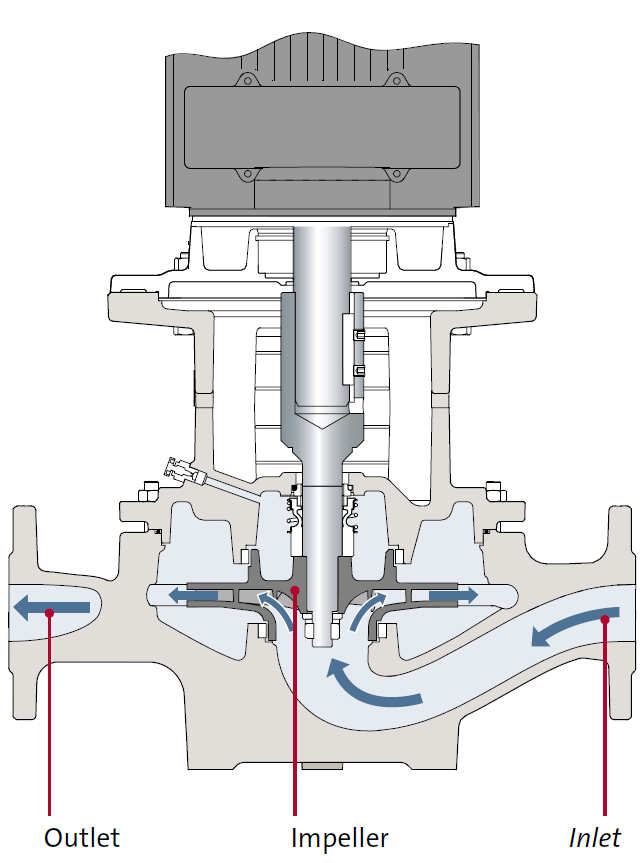
\includegraphics[width=0.4\linewidth]{figures/pump_cross_section.PNG}
    \qquad
    \hfill
    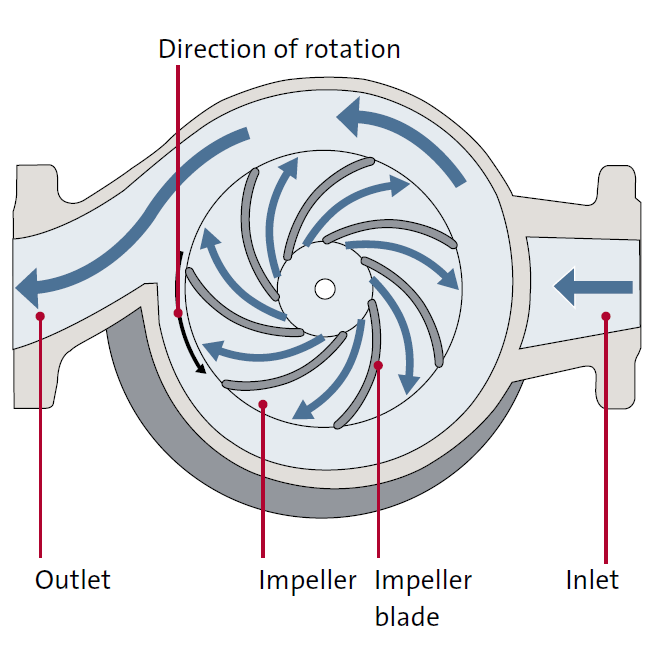
\includegraphics[width=0.4\linewidth]{figures/pump_above_view.PNG}
    \caption{Centrifugal Pump}
    \label{fig:pump_sections}
\end{figure}

\subsection{Affinity Laws}
Affinity laws are mathematical relationships that provide a way to estimate the changes in performance of a pump, as a result
of a change in one of the basic pump variables.
In it's simplest form, the term law, means a principle that has been proven true for all cases.
\todo[color=03physicalSetup]{"proven true for all cases"? that can't be correct for an estimate}

\begin{align}
	\left(\frac{N_1}{N_2}\right)^1 = \frac{Q_1}{Q_2} &&
	\left(\frac{N_1}{N_2}\right)^2 = \frac{H_1}{H_2} &&
	\left(\frac{N_1}{N_2}\right)^3 = \frac{P_1}{P_2}	
\end{align} 
Equations for constant impeller diameter $D$ \cite{AffinityLaws}


\begin{align}
	\left(\frac{D_1}{D_2}\right)^1 = \frac{Q_1}{Q_2} &&
	\left(\frac{D_1}{D_2}\right)^2 = \frac{H_1}{H_2} &&
	\left(\frac{D_1}{D_2}\right)^3 = \frac{P_1}{P_2}	
\end{align} 
Equations for constant rotational speed $N$ \cite{AffinityLaws}
\newpage

\subsection{Performance Curves}
\subsubsection{Pump Head Curve}
A QH-curve or pump curve defines the head as a function of the flow. The flow is the rate of the fluid going through the 
pump. It is generally stated in cubic meter per hour $[m^{3}/h]$. Figure \ref{fig:pump_head_curve} represents a typical pump head curve.

\begin{figure}[h]
	\centering
	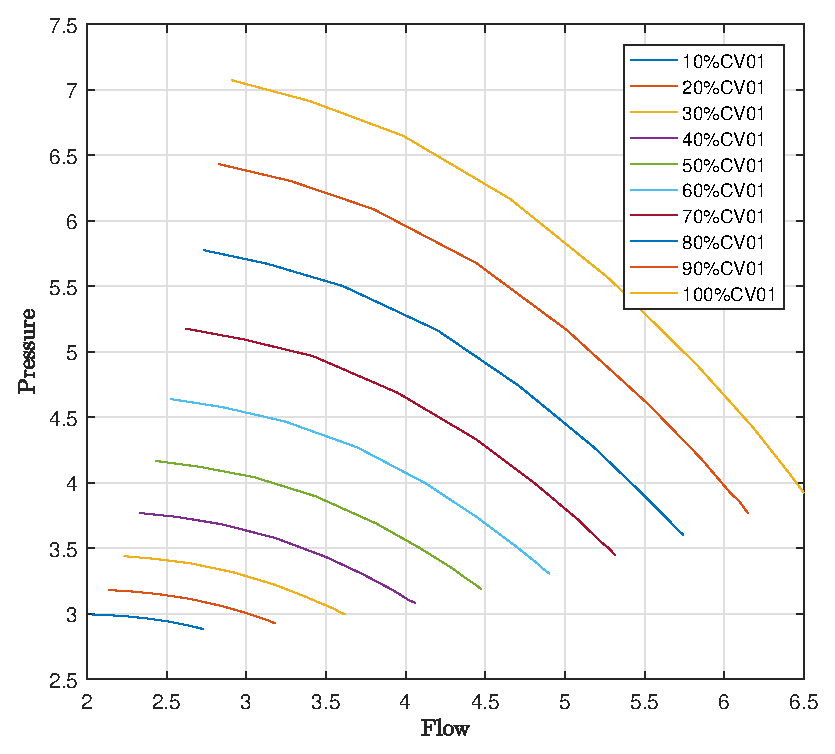
\includegraphics[width=0.4\textwidth]{figures/05mathematicalModeling/pumpCurves.eps}
	\caption{Pump Head Curve}
	\label{fig:pump_head_curve}
\end{figure}


\subsubsection{System Head Curve}
A system head curve is a graphical representation of the pump head that is required to move fluid through a piping system at various flow rates.
The system curve helps quantify the resistance in a system due to friction and elevation change over the range of flows.

Simply put, the system curve shows how much resistance the pump has to overcome in order to be able to move a certain amount of fluid though the system.
As stated before, the resistance can come from friction with the pipes, or elevation changes.
\todo[color=04mathematicalModelling]{repetitive, choose one that you think explains it the best}
\todo[color=04mathematicalModelling]{insert system curve photo}


\section{Pipes}
Pipes are a way of transporting liquids or gasses, inside a controllable environment.
They are used to interconnect the pumps and the tank and other peripherals.
One common analogy compares them to wires in electrical circuits.

Based on their diameters, material and shape,
they introduce resistance to the flow of the pumped medium.
Staying with the analogy to electrical circuits,
this can be compared to the cross sectional area and the specific resistance of a wire material.

\section{Valves}
A valve is a device used to regulate the flow of a gas or liquid through a piping system.
The valve built into our system is not used for regulatory purposes,
but only to simulate disturbances in the system.
Valves can be actuated by different means, such as air pressure, electric motors or rotary handles.

\section{Sensors}
To be able to monitor the system closely, different sensors are used.
\todo[color=03physicalSetup]{write about the sensors used in the system}

\subsection{Flow Meter}
\subsection{$\Delta$Pressure Sensor}
\subsection{Power Sensor}
\todo[color=03physicalSetup]{complete this list of subsections}
\todo[color=03physicalSetup]{maybe take out of ToC? (subsection*)}

\todo[color=03physicalSetup]{Do we want a section about xPC and Simulink Realtime?}

\chapter{Mathematical Modelling}\label{ch:mathmodel}

\section{Pump Curves}\label{sec:pumpcurves}
With the data gathered through the experiments (Section \ref{sec:experiment}\todo{not linked yet}),

\todo{re-write this section, all math used here doesn't apply to real life. But use the knowledge we gained here instead of deleting everything}
We decided to use black-box modelling with polynomial fitting.
For this we used the Curve Fitting Tool \cite{cftool} \todo{add to bibliography} \textit{cftool} \todo{make this look like a command} in MATLAB.
Looking at the data we decided to use polynomial fitting with a second degree polynomial
as can be seen in equation \ref{eq:polynom}.

\begin{equation}
	 P(Q) = p_1 \cdot Q^2 + p_2 \cdot Q + p_3
	 \label{eq:polynom}
\end{equation}

After repeating this process over different datasets with different pump speeds,
we noticed that the coefficients $p_1$ and $p_2$ barely change.
\todo{they fucking do, shit isn't even properly linear...}

The standard deviation for the $p_1$ and $p_2$ coefficients were calculated with the equation \todo{add reference to eq}

\begin{equation}
	\sigma_{\mean{p_{1,2}}} = \dfrac{1}{n}\sum |p_{1,2}-\mean{p_{1,2}}|
	\label{eq:avedev}
\end{equation}

The results obviously vary between runs. For the run used to create the model the $\sigma_{\mean{p_{1,2}}}$ are:
\begin{equation}
	\sigma_{\mean{p_1}} \simeq 0.003854$$
	
	$$\sigma_{\mean{p_2}} \simeq 0.042299
\end{equation}

The $p_3$ coefficient however changes significantly, through different pump speeds.
With a standard deviation $\sigma_{\mean{p_3}} \simeq 3.378111$ it was impossible to use only one simple polynomial as described in \ref{eq:polynom} to describe all pump characteristics at all speeds.

We were able to identify a second order polynomial describing the change in $p_3$ according to the pump speed $\omega$.
\begin{equation}
	 p_3 = a \cdot \omega^2 + b \cdot \omega + c
	 \label{eq:p3olynom}
\end{equation}

Combining \ref{eq:polynom} and \ref{eq:p3olynom}, we get:

\begin{equation}
	P(Q) = p_1 \cdot Q^2 + p_2 \cdot Q + a \cdot \omega^2 + b \cdot \omega + c 
\end{equation}
\chapter{Experiments and Lab Work}\label{ch:experiment}
Introduction goes here... 
 
\section{Performance test}\label{sec:performance_test} 
For gathering data about the pump system, a performance test was carried out.
\todo{Should we explain how a performance test is carried out?}

Instead of relying on performance curves provided by the pump manufacturer,
the pump will be run in situ, and the obtained data will show how the pump 
operates for the specific system.
 
During the test gauges for flow, pressure, speed, and power consumption were 
measured. Flow resistance can be varied by a choke valve, resulting in 
corresponding values of flow, differential pressure, and power consumption 
which has been measured in order to create the performance curves.
 
The actual code for the pump test application was done in Matlab. 
A model of the system was made using Simulink blocks. \todo{elaborate on this?}
Simulink Real-time and xPC Target was used to run the model in real-time 
on the pump system's dedicated PC. 
\todo{move somewhere else?} 

xPC Target allows you to add I/O blocks to your model, and then use the host 
PC and a C compiler to create executable code. The executable code is download 
from the host PC to the target PC running the xPC Target real-time kernel. 
After downloading the executable code, you can run and test your target 
application in real-time. \todo{nescesarry?}

% The physical system and what sensors/variables avaliable should already be explained 
- Experiment setup (What are we controlling and doing - explain the script)
- Data acquisition (other topic now?)
- Results
\todo{Do we need the datasheet for the pump? We must be using it for something?? (NPSHR?)}
 
\chapter{Model Validation and Performance}\label{ch:modValPerf}
\todo[color=06modelValidationAndPerformance]{Model Validation and Performance}
To validate the model acquired in \ref{ch:mathmodel},
we ran a second test with the same test setup as described in \ref{ch:experiment}.

\todo[color=06modelValidationAndPerformance]{create figures that compare model to data}
\missingfigure{comparison between predictions and test data}

Comparing the simulated results with the gathered data,
we get a fit of \todo[color=06modelValidationAndPerformance]{calculate fit and put here} something.


\chapter{Controller Design}\label{ch:controldesign}
\todo[color=07controllerDesign]{Controller Design not enough text yet}
\todo[color=07controllerDesign]{Explain what PID is}
\section{Step response}
\begin{figure}[H]
    \centering
    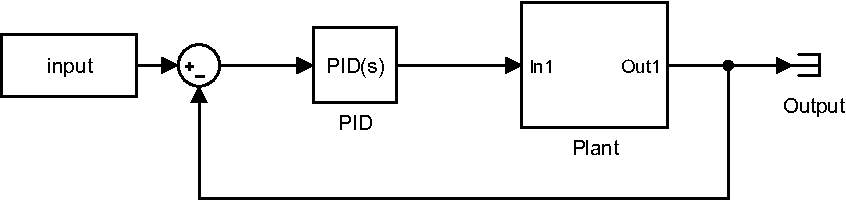
\includegraphics[width=0.75\textwidth]{figures/04ExperimentsAndLabWork/CLblock.pdf}
    \caption{A simplified block diagram to show the placement of a PID}
	\label{fig:PIDplace}
\end{figure}

For the common PID-tuning method as described by Ziegler and Nichols,
some knowledge about the system is needed.
There exist two Ziegler Nichols methods,
depending on the open-loop dynamics of the system.
Because our system has a stable response to a step input, we used the first method described in \todo[color=07controllerDesign]{page 226 ff, Feedback Control of Dynamic Systems}
Here typically a unit step input is given into the OL system as shown in figure \ref{fig:OL}.

\todo[color=07controllerDesign]{get actual values for R and L}
\begin{figure}[H]
    \centering
    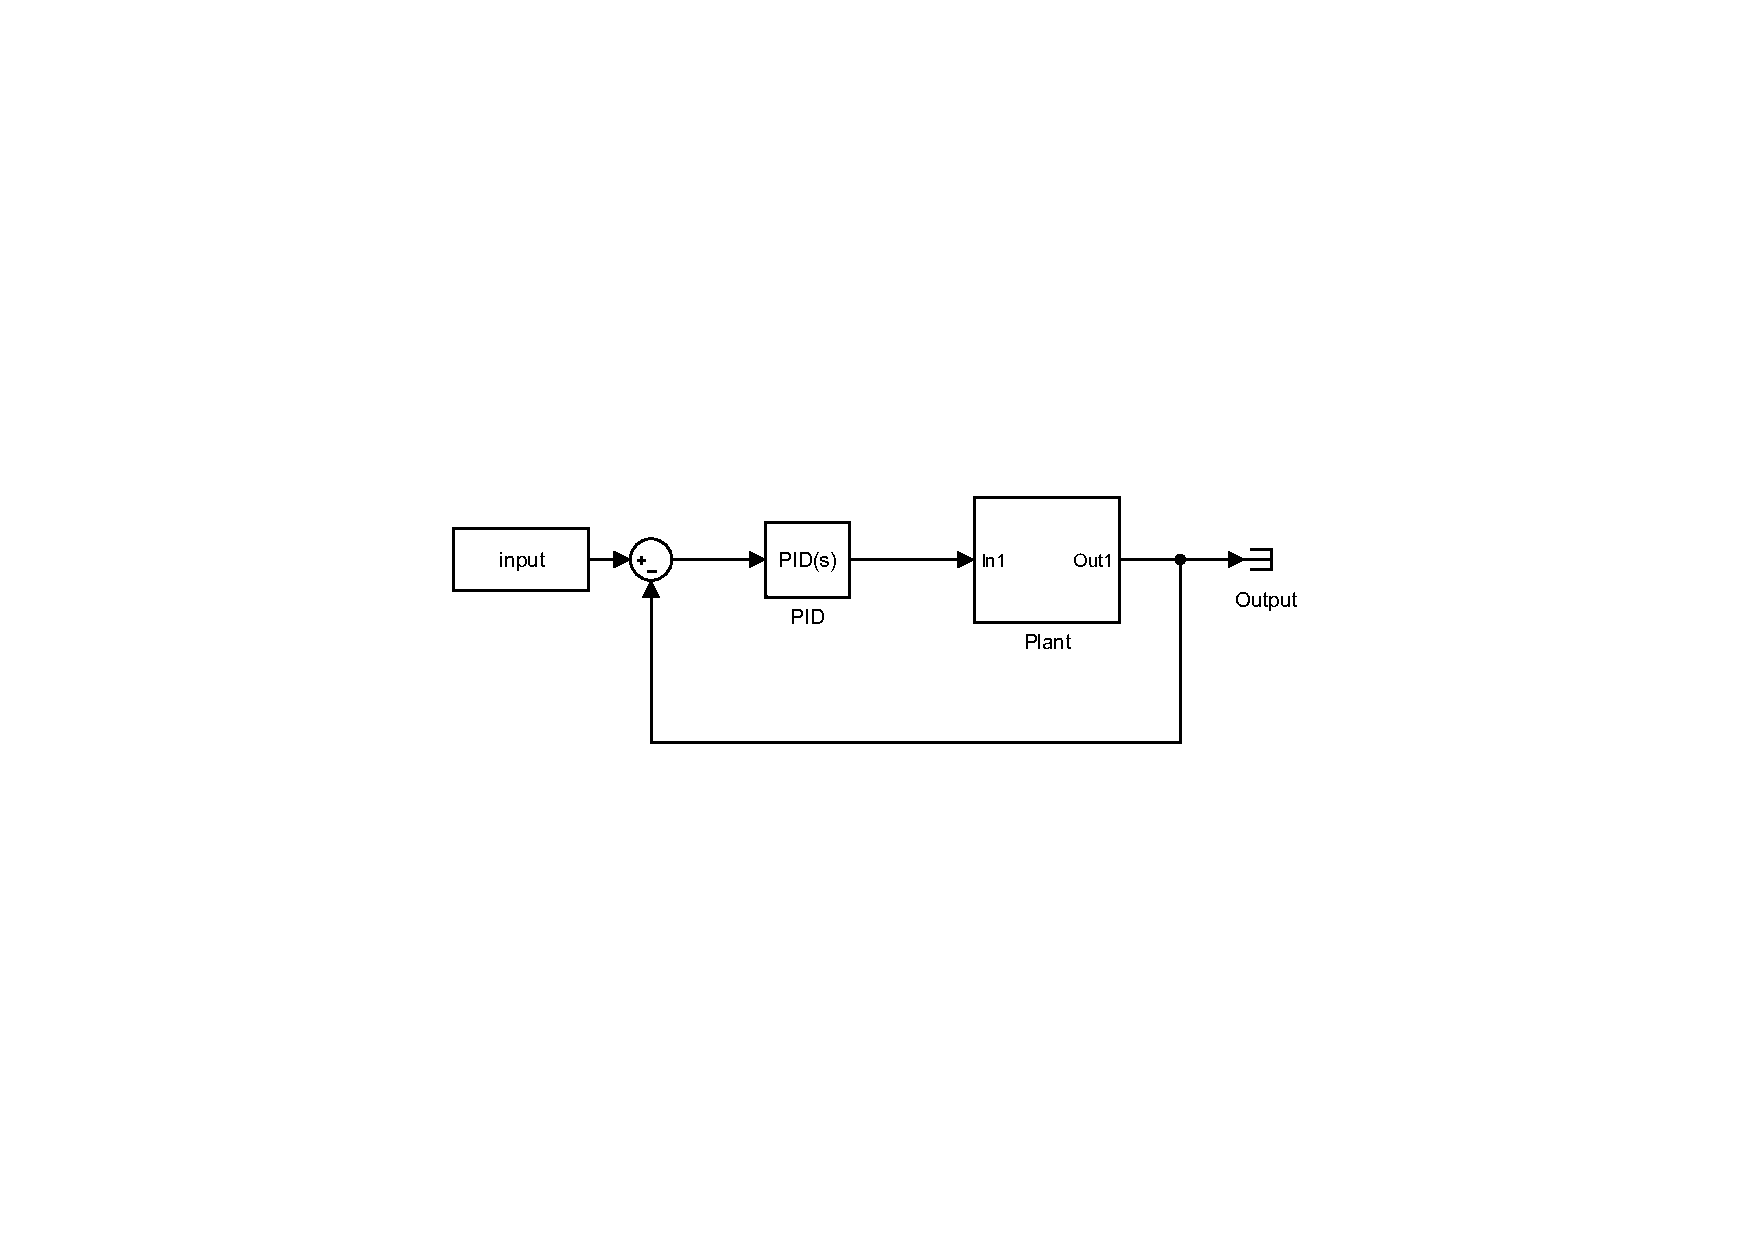
\includegraphics[width=0.75\textwidth]{figures/04ExperimentsAndLabWork/OLblock.pdf}
    \caption{OL block diagram of the system}
\label{fig:OL}
\end{figure}

Because we are scaling the $\omega$ down by a factor of 10, so we can directly read the percentage,
we had to scale the aforementioned unit step up by a factor of 10,
in order to get usable results.
While encountering this problem, we also noticed, that the pumps don't spin below an $\omega$ of 9\%.
When using the corrected step input, we got the measurements shown in figure X \ref{fig:stepin}.

Our analysis of figure \ref{fig:stepin} gives us the following values:
\\
\begin{tabular}{r c l l}
	$A$ 	& $=$ & $2.2177$ 	& \footnotesize{\textit{final value}}\\
	$R$ 	& $=$ & $1.7833$ 	& \footnotesize{\textit{slope}}\\
	$t_d=L$	& $=$ & $0.75$ 		& \footnotesize{\textit{lag}}\\
	$\tau$ 	& $=$ & $1.2436$ 	& \footnotesize{\textit{time constant}}
\end{tabular}
\\
Ziegler-Nichols is tuning a PID controller $D_c(s)$ with the formula\\
$D_c(s)=k_P(1+ \frac{1}{T_Is}+T_Ds)$,
where $k_P$, $T_I$ and $T_D$ are scalar gains,
tuned according to the characteristics obtained from figure \ref{fig:stepin}.

\begin{tabular}{r c l l}
	$k_p$ & $=$ & $\nicefrac{1.2}{RL}$	& \footnotesize{\textit{proportional gain}}\\
	$T_I$ & $=$ & $2L$					& \footnotesize{\textit{integral gain}}\\
	$T_D$ & $=$ & $0.5L$ 				& \footnotesize{\textit{derivative gain}}\\
\end{tabular}


\begin{figure}[H]
    \centering
    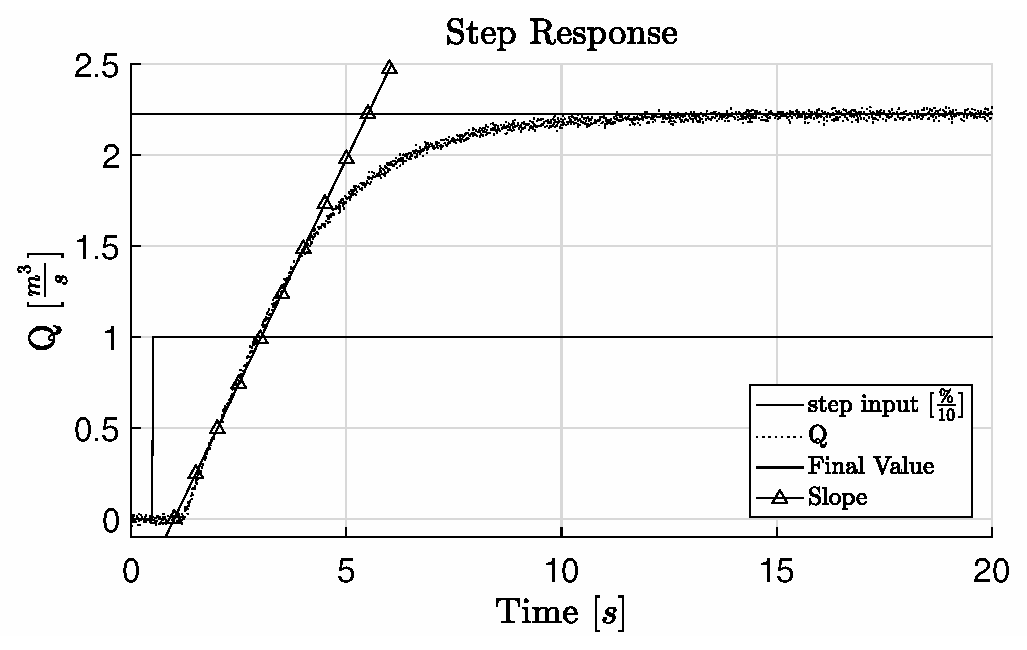
\includegraphics[width=\textwidth]{figures/04ExperimentsAndLabWork/StepResponseLabeled.eps}
    \caption{response to a step input with value 10}
	\label{fig:stepin}
\end{figure}
\todo[color=07controllerDesign]{can we make the axis look like they are made by LaTeX as well?}
\\ \\ \\ \\
\todo[color=07controllerDesign]{structure}
\chapter{Controller Implementation}\label{ch:cimplement}
\todo[color=08controllerImplementation]{no text yet}
\chapter{Discussion}\label{ch:discussion}
\todo[color=09discussion]{no text yet}
\chapter{Conclusion}\label{ch:conclusion}
\todo[color=10conclusion]{Conclusion no text yet}
\chapter{Data Aquisition}\label{ch:dataAq}

\printbibliography[heading=bibintoc]
\label{bib:mybiblio}
\appendix
\end{document}
